\chapter{Projeto - Parte 4}\label{ch:projeto-parte4}

Nesta parte do projeto, foram abordados conceitos de planeamento e aprendizagem automática, através da implementação de um agente deliberativo com procura em espaços de estados (PEE) e com processos de decisão de Markov (PDM).

Foi utilizado o mesmo ambiente da parte 2, que consiste num espaço bidimensional com dimensões fixas onde existem alvos e obstáculos, e onde o agente tem por objetivo recolher os alvos e evitar os obstáculos.

Como pode ser observado na figura~\ref{fig:agente-delib-pee}, o agente deliberativo utiliza uma estratégia de procura em espaços de estados para encontrar o caminho ideal até os alvos.
Essa abordagem permite ao agente planear suas ações com base na exploração de diferentes estados possíveis do ambiente.

Por outro lado, a figura~\ref{fig:agente-delib-pdm} mostra o agente deliberativo utilizando processos de decisão de Markov.
Esta abordagem faz uso de modelos probabilísticos para decidir a melhor ação a ser tomada em cada estado, tendo em conta a possível incerteza do ambiente.

\begin{figure}[H]
    \begin{center}
        \resizebox{100mm}{!}{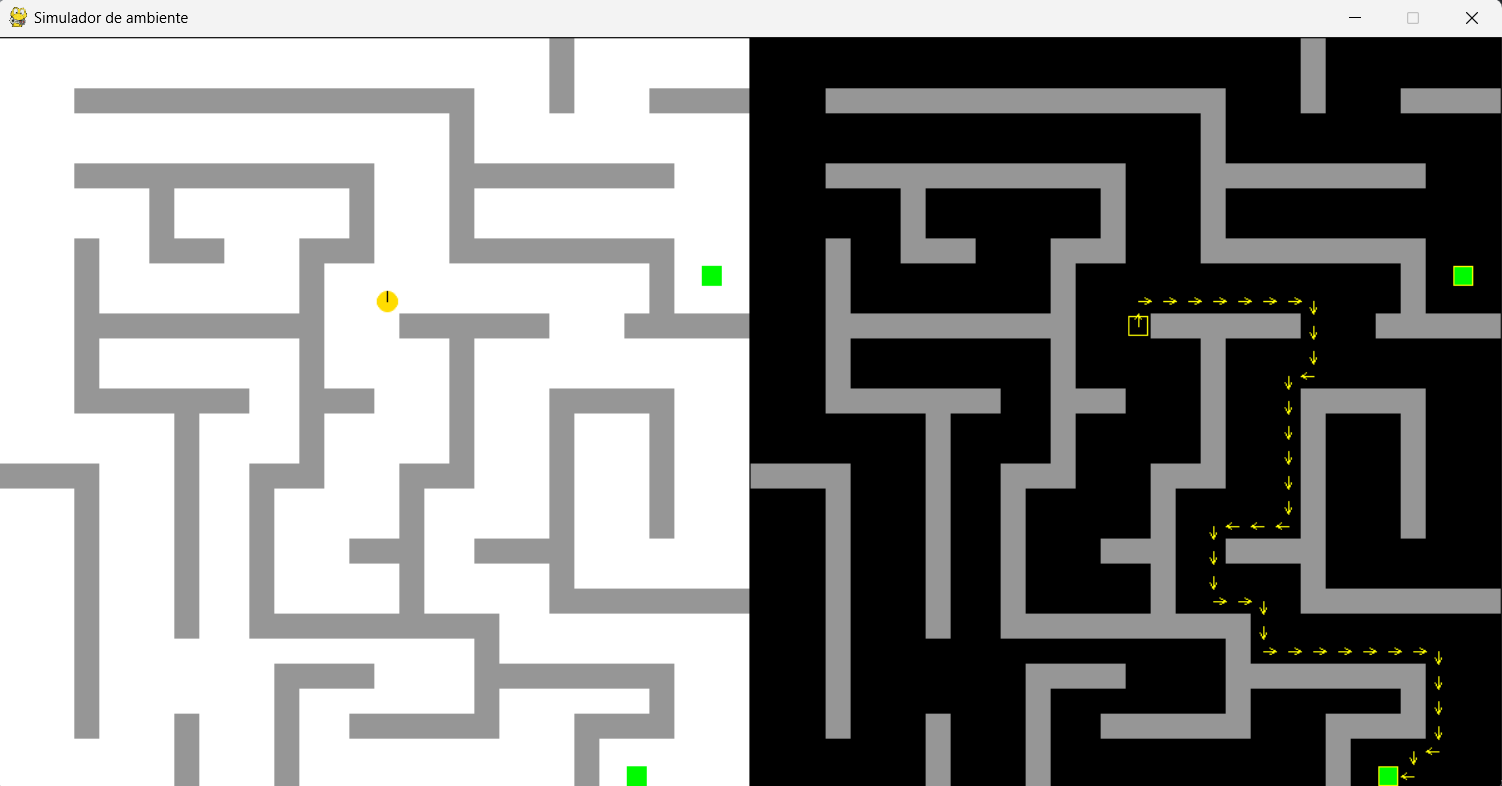
\includegraphics{../figures/agente-delib-pee}}
    \end{center}
    \caption{Agente deliberativo com procura em espaços de estados.}
    \label{fig:agente-delib-pee}
\end{figure}

\begin{figure}[H]
    \begin{center}
        \resizebox{100mm}{!}{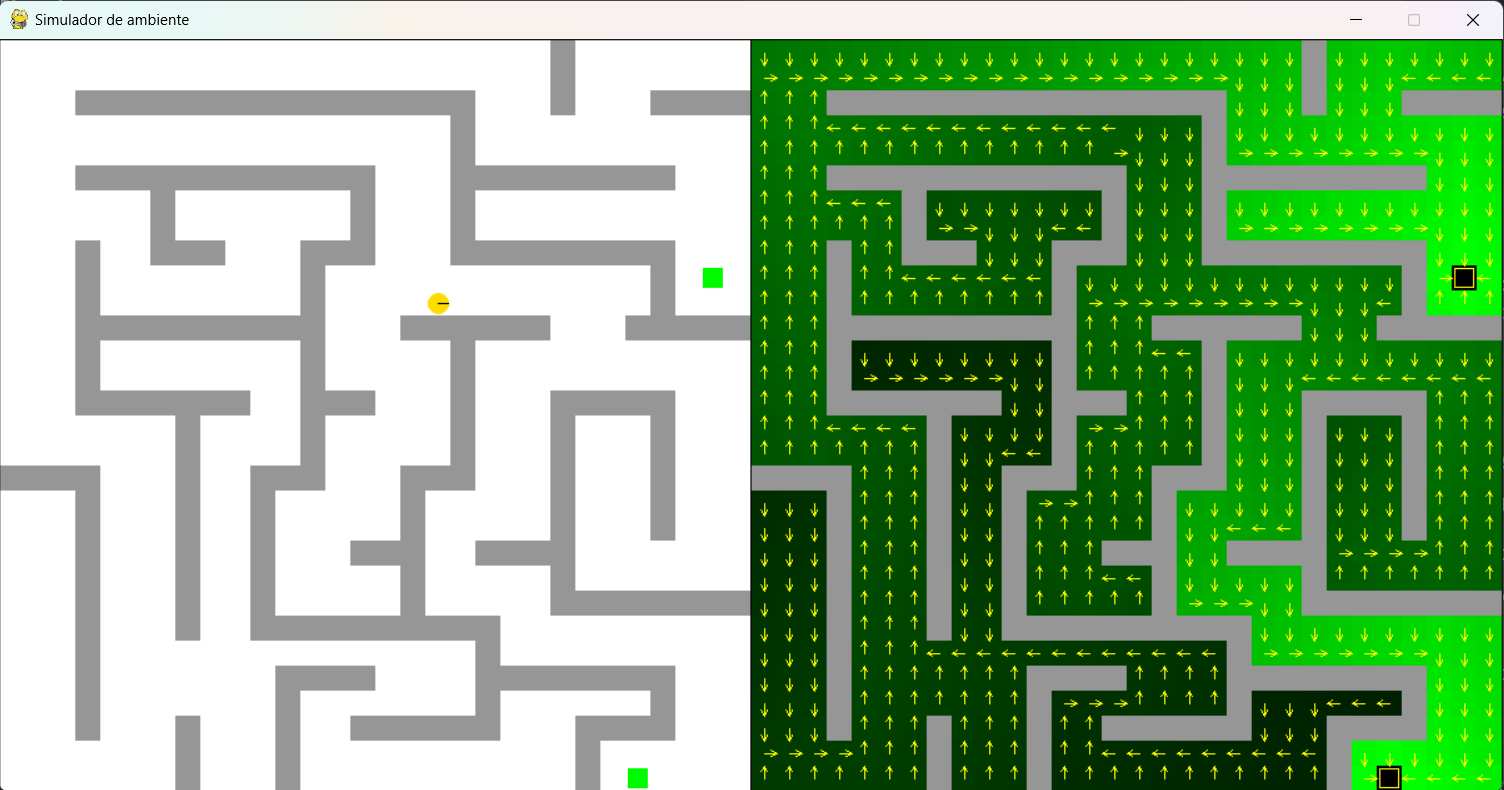
\includegraphics{../figures/agente-delib-pdm}}
    \end{center}
    \caption{Agente deliberativo com procura por processos de decisão de Markov.}
    \label{fig:agente-delib-pdm}
\end{figure}

Para que o agente possa atingir os objetivos propostos, foi necessário implementar uma arquitetura deliberativa, que permite antecipar ao agente analisar o ambiente e antecipar o futuro, de forma a planear as ações a serem tomadas.

Tal como em fases anteriores, a implementação foi feita com base na consulta e compressão de diagramas UML e de sequência de forma a garantir a correta implementação dos diferentes subsistemas.


\section{Arquitetura Deliberativa}\label{sec:arquitetura-deliberativa}

Conforme foi abordado na secção~\ref{sec:arquiteturas-reativa-memoria}, um agente reativo com memória age com conhecimento do presente, através de reações a estímulos, e com conhecimento do passado, através da memorização de percepções e de ações passadas.
Um agente deliberativo, além de possuir as características de um agente reativo com memória, é capaz de antecipar o futuro, através da simulação de cenários, e consequentemente de planear ações futuras, com base em objetivos explícitos (fixos ou gerados dinamicamente) e em processos de deliberação sobre que objetivos concretizar e quais os meios a utilizar.

Qualquer sistema para poder antecipar o futuro tem que ter conhecimento (modelo do mundo), e esse conhecimento pode ser adquirido através da experiência ou de algo que já tenha esse conhecimento e o transmita para o agente (e.g., num ambiente multi-agente, um agente pode adquirir conhecimento de outro agente).
O modelo do mundo caracteriza-se como um caso particular da representação do modelo do problema, e permite simular para cada opção as múltiplas sequências de evolução possíveis, através de uma simulação interna~\cite{isel:iasa:slides:arq-agentes-deliberativos}.

A sequência de ações geradas por um agente deliberativo, através de processos internos, caracterizam o seu comportamento, ao contrário dos agentes reativos que têm comportamentos baseados em reações.

Numa arquitetura deliberativa, o módulo de memória é indispensável e dá suporte à simulação interna e aos mecanismos de deliberação~\cite{isel:iasa:slides:arq-agentes-deliberativos}, conforme representado na figura~\ref{fig:arquitetura-deliberativa}.

\begin{figure}[H]
    \begin{center}
        \resizebox{100mm}{!}{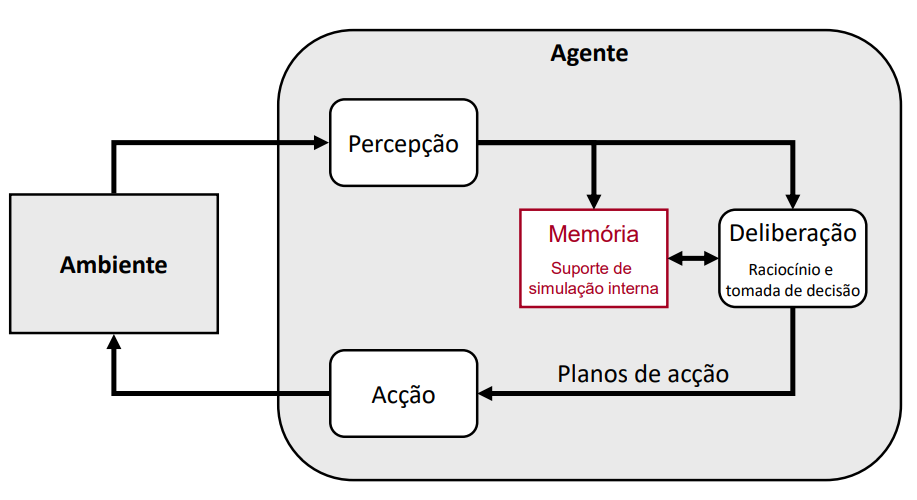
\includegraphics{../figures/arquitetura-deliberativa}}
    \end{center}
    \caption{Arquitetura deliberativa.
    Retirado de~\cite{isel:iasa:slides:arq-agentes-deliberativos}, slide 16.}
    \label{fig:arquitetura-deliberativa}
\end{figure}


\section{Raciocínio Automático}\label{sec:raciocinio-automatico-1}

Conforme foi abordado na secção~\ref{sec:raciocinio-automatico}, o raciocínio automático é um processo de inferência que permite a um agente deliberativo deduzir novas informações a partir de conhecimento prévio.

Com base nos conhecimentos adquiridos nesta fase do projeto, este raciocínio pode ser subdividido em dois tipos:

\begin{itemize}
    \item \textbf{Raciocínio Prático}: orientado para a ação (interação permanente com o mundo, ao qual está associado o processo de tomada de decisão).
    Tem como input os objetivos a atingir, as ações realizáveis e a representação do mundo, e como output os planos de ação.
    \item \textbf{Raciocínio Teórico}: orientado para o conhecimento, que permite deduzir novas informações a partir de conhecimento prévio.
    Caracteriza-se por ser direto, ou seja, não envolve interação com o mundo.
\end{itemize}

\subsection{Raciocínio Prático}\label{subsec:raciocinio-pratico}

Numa arquitectura deliberativa, o raciocínio prático suporta o processo
geral de tomada de decisão que determina o comportamento do agente,
ou seja, quais as acções a realizar perante as percepções obtidas e o
estado do modelo interno do mundo~\cite{isel:iasa:slides:arq-agentes-deliberativos}.
Este processo de tomada de decisão é composto por duas fases:

\begin{itemize}
    \item \textbf{Deliberação}: raciocínio sobre os fins, que permite definir os objetivos a atingir (i.e., opções (input) -> objetivos (output)).
    \item \textbf{Planeamento}: raciocínio sobre os meios, que permite definir os planos de ação a executar (i.e., ações (input) -> planos (output)).
\end{itemize}

Tendo em conta que o raciocínio prático é um processo de tomada de decisão, é necessário que o agente tenha objetivos, que são os critérios de avaliação das ações, e que possa avaliar as ações possíveis, de forma a escolher a melhor ação a executar.
Portanto, a deliberação sobre a representação do modelo do mundo que permite definir os objetivos, e o planeamento com base nesses e nos meios disponíveis, definem os processos necessários para a geração de planos de ação, conforme representado na figura~\ref{fig:delib-planeamento}.

\begin{figure}[H]
    \begin{center}
        \resizebox{100mm}{!}{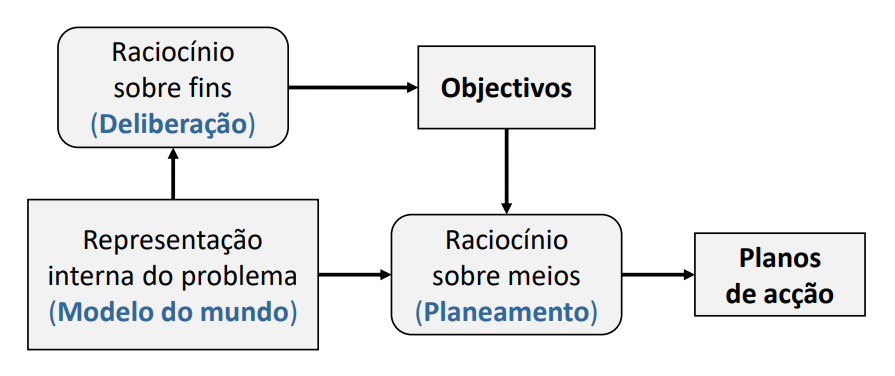
\includegraphics{../figures/delib-planeamento}}
    \end{center}
    \caption{Deliberação e planeamento num agente deliberativo.
    Retirado de~\cite{isel:iasa:slides:arq-agentes-deliberativos}, slide 8.}
    \label{fig:delib-planeamento}
\end{figure}

No entanto, o ambiente pode ser dinâmico, e por isso o agente pode ter que reagir a mudanças no ambiente (i.e., alterações no modelo do mundo), o que implica que o processo de tomada de decisão seja adaptativo, ou seja, que possa ser reavaliado e ajustado (reconsideração).
Além disso, mesmo sem alteração do estado do ambiente, o próprio plano de ação pode estar desfasado da realidade aquando da sua conceção, devido a um acontecimento que não foi antecipado (e.g., um camião que seguia um trajeto específico, mas por causa de areia no caminho, teve que mudar de trajeto).

Portanto, tanto a alteração do mundo como a dessincronização do plano de ação em relação à realidade, levam a uma reconsideração do processo de tomada de decisão.
Este processo de tomada de decisão, que ocorre de forma cíclica, pode ser então representado pelos seguintes passos~\cite{isel:iasa:slides:arq-agentes-deliberativos}:

\begin{enumerate}\label{enum:processo-tomada-decisao}
    \item Observar o mundo, gerando percepções.
    \item Atualizar o modelo do mundo, com base nas percepções.
    \item Se reconsiderar, então:
    \begin{enumerate}
        \item Deliberar o que fazer, gerando um conjunto de objetivos.
        \item Planear como fazer, gerando um plano de ação.
    \end{enumerate}
    \item Executar o plano de ação.
\end{enumerate}

\subsection{Racionalidade Limitada}\label{subsec:racionalidade-limitada}

A racionalidade limitada é um conceito que se aplica a agentes que têm recursos computacionais limitados (i.e., tempo de computação, memória), e que por isso não conseguem gerar planos de ação ótimos.

Um agente com racionalidade limitada tenta chegar a uma solução satisfatória, não à melhor solução, de forma dinâmica, tendo em conta os recursos computacionais disponíveis.
Divide o problema em subproblemas mais simples, aplicando restricções de forma a reduzir a complexidade do problema, e resolve-os sequencialmente, de forma a atingir o objetivo final~\cite{isel:iasa:slides:arq-agentes-deliberativos}.

Para o contexto humano, não é possível fazer raciocínio ótimo mas sim automático, devido à racionalidade limitada.


\section{Planeamento Automático}\label{sec:planeamento-automatico}

O planeamento automático é um processo deliberativo, que faz parte do raciocínio prático,
que tem por objetivo
gerar sequências de ação, designadas planos~\cite{isel:iasa:slides:plan-autom-pee}.
Um processo de planeamento requer um modelo de planeamento que define a representação abstrata do problema a resolver, e que apresenta os mesmos conceitos que foram abordados na secção~\ref{subsec:modelacao-problema} (i.e., estados, operadores, etc...).
Dado um modelo de planeamento e um conjunto de objetivos provenientes do processo de deliberação, o planeador gera um plano de ação que permite ao agente concretizar esses objetivos.

Este processo é realizado através de métodos de raciocínio automático, como a procura em
espaço de estados e a procura por processos de decisão de Markov~\cite{isel:iasa:slides:plan-autom-pee}.

\subsection{Planeador Baseado em PEE}\label{subsec:planeador-baseado-em-pee}

No caso de um planeador baseado em procura em espaços de estados (PEE), é necessário considerar~\cite{isel:iasa:slides:plan-autom-pee}:

\begin{itemize}\label{itemize:planeador-baseado-em-pee}
    \item Modelo do problema de planeamento.
    \item Heurística a utilizar (se necessário) para guiar a procura (ver secção~\ref{subsubsec:heuristica}).
    \item Mecanismo de procura (ver secção~\ref{sec:mecanismo-procura}).
\end{itemize}

\subsection{Planeador Baseado em PDM}\label{subsec:planeador-baseado-em-pdm}

No caso de um planeador baseado em processos de decisão de Markov (PDM), a representação do domínio do problema é feita sobre a forma de um processo de decisão de Markov, que se define como um modelo matemático que descreve um sistema que evolui ao longo do tempo, com base em estados e ações, e que é utilizado para modelar situações de decisão sequencial sob incerteza~\cite{isel:iasa:slides:plan-autom-pdm}.

Ao contrário do planeador baseado em PEE, o planeador baseado em PDM não gera um plano de ação, mas sim uma política.
Esta política define-se como uma função que mapeia estados em ações, e que é utilizada para determinar a ação a executar em cada estado, definindo a estratégia de tomada de decisão do agente.

Além disso, em vez de só ter em conta o custo, o planeador baseado em PDM tem em conta a utilidade de uma ação que depende de uma sequência de decisões, da possibilidade de ganhos e perdas, da incerteza na decisão e do efeito cumulativo~\cite{isel:iasa:slides:processos-decisao-sequencial}.


\section{Processos de Decisão Sequencial}\label{sec:processos-de-decisao-sequencial}

No processo de decisão geral, cada estado $s$ é caracterizado por um conjunto de atributos que descrevem o estado do mundo, e cada ação $a$ é uma transformação que altera o estado do mundo, levando a um novo estado $s'$~\cite{isel:iasa:slides:processos-decisao-sequencial}.
O valor (utilidade) desses estados e decisões pode não ser conhecido de imediato, sendo percebido apenas de forma diferida no tempo, devido a potenciais encadeamentos de estados e possíveis decisões futuras, conforme representado na figura~\ref{fig:processo-decisao-sequencial}.

No processo de decisão sequencial, a evolução entre estados ocorre por efeito de ações que, no caso geral, podem ser não deterministas, ou seja, o resultado das ações pode não ser completamente previsível, podendo existir incerteza no seu resultado.
Esse tipo de processos corresponde a espaços de estados (ambientes) não deterministas (estocásticos), nos quais as transições entre estados ocorrem por efeito das ações, cada uma com uma probabilidade associada de forma a representar a incerteza do ambiente. A cada transição pode estar associada uma recompensa, que representa o ganho ou perda relacionado a essa transição de estado~\cite{isel:iasa:slides:processos-decisao-sequencial}.

\begin{figure}[H]
    \begin{center}
        \resizebox{100mm}{!}{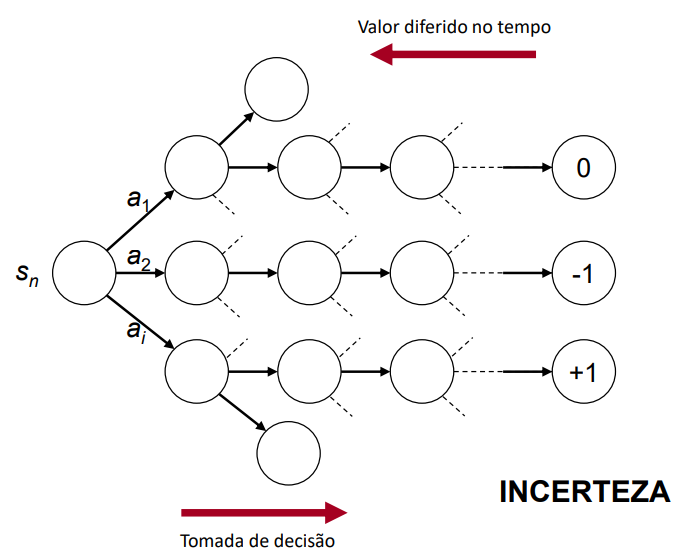
\includegraphics{../figures/processo-decisao-sequencial}}
    \end{center}
    \caption{Processo de decisão sequencial.
    Retirado de~\cite{isel:iasa:slides:processos-decisao-sequencial}, slide 3.}
    \label{fig:processo-decisao-sequencial}
\end{figure}


\section{Cadeias de Markov}\label{sec:cadeias-de-markov}

Uma cadeia de Markov~\cite{wiki:markov-chain} é um processo estocástico que evolui ao longo do tempo, com
base em estados e transições entre esses estados, e que obedece à propriedade de Markov~\cite{isel:iasa:slides:processos-decisao-sequencial}.

A propriedade de Markov é uma propriedade em processos estocásticos, que se caracteriza pela distribuição probabilística condicional dos estados futuros de um processo depender exclusivamente do estado presente (i.e., a previsão dos estados seguintes só depende do estado presente)~\cite{isel:iasa:slides:processos-decisao-sequencial}.

Formalmente, uma cadeia de Markov é definida por um conjunto de estados $S$ e por uma função de transição $T$, que define a probabilidade de transição de um estado para outro,
conforme representado na figura~\ref{fig:cadeia-de-markov}.

\begin{figure}[H]
    \begin{center}
        \resizebox{100mm}{!}{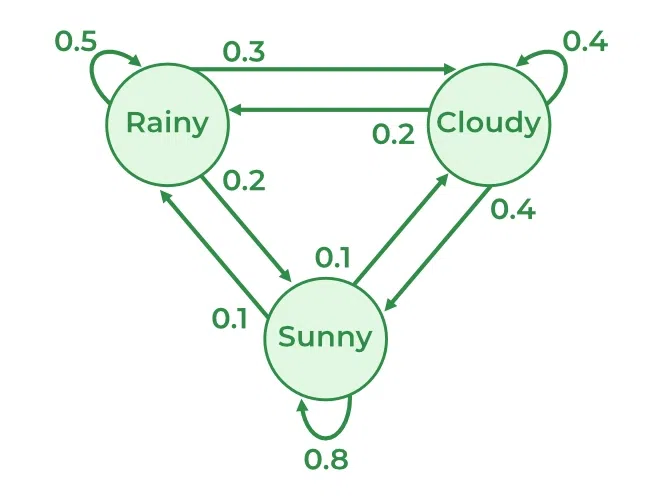
\includegraphics{../figures/cadeia-markov}}
    \end{center}
    \caption{Cadeia de Markov.
    Retirado de~\cite{isel:iasa:slides:processos-decisao-sequencial}, slide 7.}
    \label{fig:cadeia-de-markov}
\end{figure}


\section{Processos de Decisão de Markov}\label{sec:processos-de-decisao-de-markov}

O processo de decisão de Markov (PDM) é um processo de controlo estocástico em tempo discreto, e que fornece um modelo matemático para modelar situações de decisão sequencial sob incerteza~\cite{wiki:markov-decision-process}.
Esta incerteza resulta da impossibilidade de se obter informação completa relativa ao domínio do problema (e.g., navegação em veículos autónomos).
Este processo caracteriza-se como uma extensão de uma cadeia de Markov, que inclui, além dos estados e transições; ações e recompensas, de forma a obter uma política.
Formalmente, é representado pelo seguinte conjunto de elementos:

\begin{itemize}\label{itemize:processo-decisao-markov}
    \item \textbf{$S$}: conjunto de estados do mundo;
    \item \textbf{$A$}: conjunto de ações possíveis no estado $s \in S$;
    \item \textbf{Modelo de transição}: \( T(s, a, s') \), onde \( s \) é o estado atual, \( a \) é a ação a ser tomada, e \( s' \) é o estado futuro.
    é a probabilidade de mudança de estado de \( s \) para \( s' \) após a ação \( a \) ser tomada.
    Em ambientes deterministas, a probabilidade de transição é 1, e em ambientes estocásticos, a probabilidade de transição é um valor entre 0 e 1;
    \item \textbf{Modelo de recompensa}: \( R(s, a, s') \), onde \( s \) é o estado atual, \( a \) é a ação a ser tomada, e \( s' \) é o estado futuro.
    é a recompensa associada à transição de estado de \( s \) para \( s' \) após a ação \( a \) ser tomada.
    Este modelo está descrito no caso geral, mas poderá estar dependente apenas do estado atual e da ação tomada ou apenas do estado atual;
    \item \textbf{Factor de desconto}: \( \gamma \), onde \( 0 \leq \gamma \leq 1 \), que é o fator de retenção aplicado à recompensa.
    Por cada unidade de tempo que passa, a recompensa é descontada por um fator de \( \gamma \), de forma exponencial.
    Se \( \gamma = 0 \), a tomada de decisão só depende do presente, porque o futuro é anulado.
\end{itemize}

\subsection{Utilidade}\label{subsec:utilidade}

O valor (utilidade) de um estado caracteriza-se com o efeito acumulativo que vai tendo do mundo, através dos ganhos e perdas que vai obtendo, diferidos no tempo, visto que pode existir perda de oportunidade na passagem do tempo (e.g., no mercado financeiro, o valor de uma ação é volátil e varia ao longo do tempo, comprar uma ação em t0 pode ser mais vantajoso do que comprar a mesma ação em t1).
No entanto, poderão existir estados em que não existem ganhos e perdas.

Portanto, a utilidade representa o valor de se estar num estado, para efeito de concretização de um objetivo do sistema, mas representa o valor a longo prazo (na história de evolução do sistema) (e.g., um automóvel pode ter que acelarar, gastando mais combustivel, para evitar um acidente, mas a longo prazo, o valor de evitar o acidente é maior do que o valor de gastar mais combustivel).

\subsection{Política}\label{subsec:politica-otima}

Uma política ($\pi$) é uma função que mapeia estados em ações, e que é utilizada para determinar a ação a executar em cada estado, definindo a estratégia de tomada de decisão do agente.
É caracterizada em dois tipos:

\begin{itemize}
    \item \textbf{Determinística}: mapeia cada estado em apenas uma ação ($\pi : S \rightarrow A(s); \quad s \in S$);
    \item \textbf{Estocástica}: mapeia cada estado numa distribuição de probabilidade sobre as ações possíveis ($\pi : S \times A(s) \rightarrow [0,1]; \quad s \in S$).
\end{itemize}

\subsection{Objetivo}\label{subsec:objetivo}

O objetivo de um processo de decisão de Markov é determinar a política ótima ($\pi^*$), que é a política que maximiza a utilidade esperada, ou seja, a política que maximiza a recompensa esperada ao longo do tempo, através das equações de Bellman~\cite{wiki:bellman-equation}.
Devido à propriedade de Markov, a utilidade de um estado dada uma ação é a soma da recompensa imediata e da utilidade esperada do estado seguinte, ponderada pelo fator de desconto $\gamma$, conforme representado na equação de Bellman~\ref{eq:bellman-utilidade-acao}.

\begin{equation}
    \label{eq:bellman-utilidade-acao}
    U(s, a) = \sum_{s'} T(s, a, s') [R(s, a, s') + \gamma U^\pi(s')]
\end{equation}

De forma a calcular a utilidade esperada de um estado, é necessário considerar a ação que maximiza a utilidade esperada desse estado, conforme representado na equação de Bellman~\ref{eq:bellman-utilidade-final}.

\begin{equation}
    \label{eq:bellman-utilidade-final}
    Ufinal(s) = \max_{a} U(s, a)
\end{equation}

A partir da utilidade esperada de cada estado, é possível determinar a política ótima ($\pi^*$), que é a política que seleciona a ação que maximiza a utilidade esperada de cada estado, conforme representado na equação de Bellman~\ref{eq:bellman-politica-otima}.

\begin{equation}
    \label{eq:bellman-politica-otima}
    \pi^*(s) = \arg\max_{a} Ufinal(s, a)
\end{equation}

\subsubsection{Algoritmo de Iteração de Valor}\label{subsubsec:algoritmo-iteracao-valor}

O algoritmo de iteração de valor é um algoritmo que permite calcular a utilidade ótima de cada estado, através da iteração de cálculos de utilidade, até que a utilidade de cada estado convirja para um valor estável.
Este algoritmo inicializa a utilidade de cada estado a zero e, de forma iterativa, calcula a utilidade de cada estado, conforme a equação de Bellman~\ref{eq:bellman-utilidade-final}, até que um determinado critério de convergência seja atingido~\cite{isel:iasa:slides:processos-decisao-sequencial}.

O critério de convergência é representado por um $\delta$, que define a diferença máxima permitida entre a utilidade atual de um estado e a utilidade do estado na iteração anterior.
À medida que as utilidades de cada estado são atualizadas ao longo das iterações, elas convergem para valores muito próximos, até que a partir de um determinado ponto são irrisórias, e consequentemente consideradas estáveis.
Isto acontece porque a política converge mais cedo que a utilidade, por isso o $\delta$ é usado para verificar a convergência da política.

O algoritmo apresenta assim 2 ciclos: um ciclo externo que controla a convergência do algoritmo, e um ciclo interno que calcula a utilidade para cada estado, conforme ilustrado na figura~\ref{fig:algoritmo-iteracao-valor}.

\begin{figure}[H]
    \begin{center}
        \resizebox{100mm}{!}{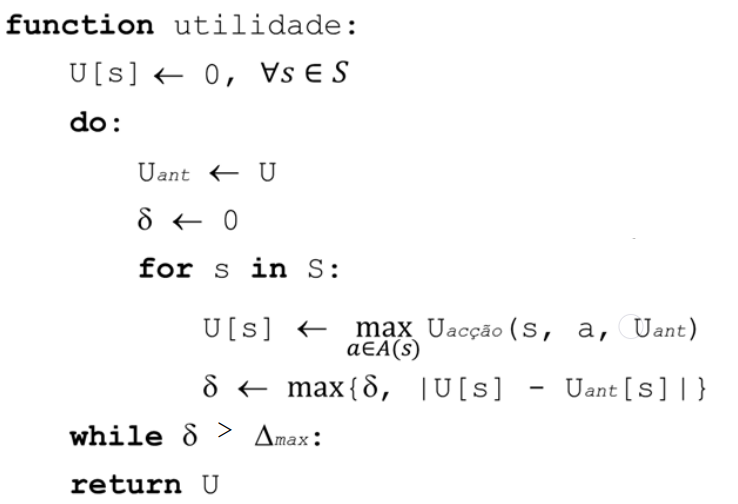
\includegraphics{../figures/algoritmo-iter-valor}}
    \end{center}
    \caption{Algoritmo de iteração de valor.
    Retirado de~\cite{isel:iasa:slides:processos-decisao-sequencial}, slide 21.}
    \label{fig:algoritmo-iteracao-valor}
\end{figure}

Também de notar que o algoritmo de iteração de valor é um algoritmo de programação dinâmica, que é uma técnica de otimização que consiste em dividir um problema em subproblemas mais simples, guardando soluções intermédias, de forma a evitar o recalculo de soluções já calculadas.


\section{Aprendizagem Automática}\label{sec:aprendizagem-automatica}

Num conceito geral, a aprendizagem define-se como a melhoria de desempenho, para uma dada tarefa, com a experiência.
Esta experiência tem por base a memória, que é o grau mais básico da inteligência. No entanto, aprender não é apenas memorizar; é ganhar a capacidade de adaptação.

A aprendizagem automática define-se como um campo da inteligência artificial que se foca no desenvolvimento de algoritmos e técnicas que permitem aos sistemas aprender a partir de dados, de forma a melhorar o seu desempenho em tarefas específicas.
Esta aprendizagem tem como base os seguintes elementos~\cite{isel:iasa:slides:aprendizagem-por-reforco}:

\begin{itemize}
    \item \textbf{Qual é a tarefa a ser aprendida (T)}: é a tarefa que o sistema tem que aprender, e que é definida pelo problema a resolver (e.g., jogar xadrez).
    \item \textbf{Métrica de desempenho (D)}: é a métrica que permite avaliar o desempenho do sistema, e que é utilizada para medir a qualidade da solução obtida (e.g., número de jogos ganhos)
    \item \textbf{Com base na experiência, como é que o sistema vai aprender (E)}: é o processo de aprendizagem, que é a forma como o sistema adquire conhecimento (e.g., jogos realizados).
\end{itemize}

Por exemplo, nas arquiteturas reativas, a aprendizagem é implícita nas associações estímulo-resposta (aprendizagem por associação), e nas arquiteturas deliberativas, a aprendizagem é explícita, através da simulação de cenários e do planeamento de ações futuras.

A aprendizagem automática divide-se em dois tipos~\cite{isel:iasa:slides:aprendizagem-por-reforco}.

\begin{itemize}
    \item \textbf{Conceptual}: Refere-se ao que o sistema aprende (e.g., aprendizagem supervisionada, aprendizagem não supervisionada);
    \item \textbf{Comportamental}: Refere-se a como o sistema aprende (e.g., aprendizagem por reforço).
\end{itemize}

\subsection{Aprendizagem por Reforço}\label{subsec:aprendizagem-por-reforco}

A aprendizagem por reforço é uma técnica de aprendizagem automática que treina software para tomar decisões de modo a obter os melhores resultados, imitando o processo de aprendizagem por tentativa e erro que os humanos utilizam para atingir os seus objetivos.
Neste tipo de aprendizagem, as ações que contribuem para o objetivo são reforçadas (i.e., recompensadas positivamente), enquanto as ações que prejudicam o objetivo são ignoradas (ou punidas) (i.e., recompensadas negativamente)~\cite{aprendizagem-por-reforco}.

Em processos de decisão de Markov, este tipo de aprendizagem é utilizado para ajudar os sistemas de inteligência artificial a obter resultados ótimos em ambientes parcialmente observáveis, estocásticos, dinâmicos ou até contínuos, onde a modelação do mundo é complexa e/ou desconhecida.
Por exemplo, a dimensionabilidade dos espaços de estados pode ser muito grande, a definição de modelos do mundo pode ser difícil tendo por base dados experimentais ou amostras, e os modelos de transição e de recompensa podem ser desconhecidos~\cite{isel:iasa:slides:aprendizagem-por-reforco}.
Por este motivo, o modelo precisa de ser construído a partir da experiência de forma incremental, nomeadamente através da tentativa e erro, com o objetivo de ajustar a política de decisão e maximizar a utilidade esperada.

\subsubsection{Aprendizagem por Valor de Ação}\label{subsubsec:aprendizagem-por-valor-acao}

A aprendizagem por valor de ação é um técnica de aprendizagem por reforço que tem por objetivo aprender a função que estima o valor de cada ação ($Q(a)$) (e.g., decisão entre várias ações com valores desconhecidos), de forma a maximizar a recompensa a longo prazo.
Esta função pode ser determinada, por exemplo, através: da escolha repetida de diferentes ações (i.e., qual o valor médio para uma ação após $n$ tentativas); da recompensa obtida por escolher uma determinada ação, de acordo com uma distribuição de probabilidades~\cite{isel:iasa:slides:aprendizagem-por-reforco}.

No entanto, a aprendizagem por valor de ação tem a desvantagem de se ter que realizar $n$ tentativas para cada ação e manter informação sobre os resultados obtidos, de forma a calcular a estimativa de valor de cada ação.
Tal abordagem pode ser ineficiente do ponto de vista de recursos computacionais, e não permitir aproveitar o conhecimento obtido de forma incremental.

Além disso, a recompensa pode variar ao longo do tempo (em distribuições não estacionárias) e por isso é necessário ajustar a função de valor de ação de forma a refletir essa variação.
A taxa de aprendizagem ($\alpha$) é um fator de ajuste que é aplicado ao erro de previsão, para ajustar a previsão de forma exponencial por cada unidade de tempo que passa, e que regula a importância das informações mais recentes em relação às informações mais antigas.

\begin{itemize}
    \item Se $\alpha = 0$, o sistema não aprende, porque o erro de previsão é anulado (i.e., maior relevância das recompensas mais antigas);
    \item Se $\alpha = 1$, o sistema aprende, porque o erro de previsão é maximizado (i.e., torna-se um agente reativo, é guiado pela recompensa imediata, maior relevância das recompensas mais recentes)~\cite{isel:iasa:slides:aprendizagem-por-reforco}.
\end{itemize}

Portanto, se o agente apenas escolher a ação que atualmente tem a maior estimativa de valor (abordagem Greedy), pode ficar preso a uma política subótima devido a máximos ou mínimos locais, sem explorar o ambiente para obter mais conhecimento.

Existe, portanto, um compromisso (trade-off) entre explorar (para obter conhecimento) e aproveitar (o conhecimento adquirido até ao momento, para maximizar a recompensa).
Uma abordagem possível para balancear este compromisso é a seleção de ações com base na política $\epsilon$-Greedy.
Nesta estratégia, o agente escolhe a ação com maior valor estimado com probabilidade $1 - \epsilon$, e escolhe uma ação aleatória com probabilidade $\epsilon$~\cite{isel:iasa:slides:aprendizagem-por-reforco}.
A ideia dessa estratégia é que, ao explorar ocasionalmente, o agente pode descobrir ações melhores do que aquelas que inicialmente acreditava serem as melhores num determinado momento, o que contribui para a melhoria da política de decisão.

O fator de exploração ($\epsilon$) regula o compromisso entre explorar e aproveitar, permitindo que, em determinados momentos, o agente explore o ambiente para obter conhecimento, e, em outros momentos, utilize o conhecimento adquirido até então para agir de forma a maximizar a recompensa.
Para convergir para o valor ótimo, um agente não pode apenas explorar nem apenas aproveitar, mas sim encontrar um equilíbrio entre os dois.
No entanto, é recomendável que a exploração seja progressivamente reduzida ao longo do tempo~\cite{isel:iasa:slides:aprendizagem-por-reforco}.

\subsubsection{Apredizagem por Diferença Temporal}\label{subsubsec:aprendizagem-por-diferenca-temporal}

A aprendizagem por diferença temporal~\cite{wiki:temporal-difference-learning} é uma técnica de aprendizagem por reforço que combina elementos de métodos de Monte Carlo e programação dinâmica.
Esta técnica tem por objetivo estimar o valor por acumulação de recompensas de forma
não linear para lidar com ambientes não estacionários (regulada pelo fator de aprendizagem $\alpha \in [0,1]$), e atualizar a estimativa de valor de estado-acção com base na sua mudança (diferença temporal) entre instantes sucessivos~\cite{isel:iasa:slides:aprendizagem-por-reforco}.

A aplicação prática da aprendizagem por diferença temporal pode ser feita através de dois tipos de algoritmos~\cite{q-learning-algorithm}:

\begin{itemize}
    \item \textbf{Off-policy}:
    Atualiza a estimativa de valor de estado-ação com base na ação que maximiza o valor do estado subsequente, independentemente da ação escolhida pelo agente (por exemplo, o algoritmo Q-Learning).
    Neste algoritmo, a política de escolha de ação, como a estratégia $\epsilon$-Greedy para exploração, determina como o agente explora o ambiente enquanto aprende.
    No entanto, a atualização dos valores de estado-ação segue uma abordagem Greedy, utilizando a melhor estimativa possível para a próxima ação.
    \item \textbf{On-policy}: Atualiza a estimativa de valor de estado-ação com base nas ações que o agente efetivamente executa de acordo com a política atual (aprendizagem incremental a partir da experiência) (por exemplo, algoritmo SARSA - State-Action-Reward-State-Action).
    Para resolver o dilema entre explorar e aproveitar, a seleção de ação no algoritmo SARSA pode ser implementada com a estratégia $\epsilon$-Greedy.
    Isso significa que o agente escolhe ações de forma $\epsilon$-Greedy enquanto continua a melhorar as suas estimativas de valor de estado-ação com base nas ações reais que executa.
\end{itemize}


\section{Implementação do Controlo Deliberativo}\label{sec:implementacao-controlo-deliberativo}

O controlo deliberativo corresponde a um componente que exerce raciocínio automático, mais concretamente, prático, e que está inserido numa arquitetura deliberativa.

Considerando que o objetivo do agente é movimentar-se num ambiente bidimensional, caracterizado conforme descrito na secção~\ref{sec:caracterizacao-ambiente}, de dimensões fixas, com obstáculos, de forma a recolher alvos, o controlo deliberativo foi implementado com base nos seguintes componentes~\cite{isel:iasa:slides:arq-agentes-deliberativos}:

\begin{itemize}
    \item \textbf{Modelo do mundo}: Corresponde às representações internas do ambiente, onde a memoria do agente é organizada internamente para poder ter a representação do domínio do problema. Neste caso, o modelo do mundo é representado por:
    \begin{itemize}
        \item \textbf{EstadoAgente}: Representa um estado possível onde o agente pode estar, que é
        caracterizado pela sua posição no ambiente.
        \item \textbf{OperadorMover}: Gera a transformação de um estado para outro.
        No contexto de um ambiente bidimensional, a passagem de uma posição para outra é feita através de um passo e uma direção (translação geométrica).
    \end{itemize}
    É também importante realçar que a alteração do mundo é apenas é detetada quando um elemento alvo é recolhido, visto que o ambiente é estático.
    \item \textbf{Mecanismo Deliberativo}: Responsável pelo processo de deliberação, que gera objetivos com base nas opções disponíveis.
    Neste contexto, os objetivos caracterizam-se pelas posições/estados no ambiente que o agente pretende alcançar, organizados pela sua distância ao agente (i.e., objetivos mais próximos têm maior prioridade).
    \item \textbf{Planeador}: Responsável por gerar planos de ação com base em objetivos.
    Foi definido de forma abstrata, de forma a poder ser utilizado tanto com a procura por espaços de estados como com processos de decisão de Markov (ver secção~\ref{sec:planeamento-automatico})
    \item \textbf{Controlo Deliberativo}: Orquestra todo o processo deliberativo com todas os componentes já mencionados, implementando o processo de tomada de decisão~\ref{enum:processo-tomada-decisao}.
\end{itemize}

\subsection{Implementação do Agente Deliberativo}\label{subsec:implementacao-agente-deliberativo}

Com a implementação do controlo deliberativo, foi possível desenvolver um agente deliberativo para ambos as procuras em espaços de estados e processos de decisão de Markov, diferenciando-se apenas na forma como o planeador é implementado.

\subsubsection{Implementação do Planeador PEE}\label{subsubsec:implementacao-planeador-pee}

O planeador para a procura em espaços de estados, que foi apresentado de forma abstrata na secção~\ref{subsec:planeador-baseado-em-pee},
apresenta a seguinte implementação:

\begin{itemize}
    \item \textbf{Modelo do problema de planeamento}: Tendo em conta que o modelo do mundo no controlo deliberativo já detém o estado e os operadores, este problema apenas representa um problema de planeamento, com um estado final a atingir (objetivo);
    \item \textbf{Heurística}: Utilizada para guiar a procura, a heurística calcula a distância euclidiana entre duas posições no plano;
    \item \textbf{Mecanismo de procura}: Foi utilizado um mecanismo de procura de melhor primeiro (ver secção~\ref{subsubsec:procura-melhor-primeiro}), de forma a não comprometer a implementação do planeador com um mecanismo de procura em concreto.
\end{itemize}

Se for encontrada solução, é criado um plano de ação que é executado pelo agente, e que é composto por uma sequência de ações que permitem ao agente concretizar os objetivos.

\subsubsection{Implementação do Planeador PDM}\label{subsubsec:implementacao-planeador-pdm}

Existem alguns pressupostos que foram considerados para a implementação deste planeador:

\begin{itemize}
    \item \textbf{Parameterização da recompensa máxima}: A recompensa máxima foi definida com um valor elevado de forma a permitir distinguir de forma clara entre situações de ganho e de perda;
    \item \textbf{Devido ao ambiente ser determinístico}, foi pré-calculado o conjunto das possíveis transições de estado, de forma a permitir a execução do planeador de forma eficiente;
\end{itemize}

O planeador para procura com processos de decisão de Markov, que foi apresentado de forma abstrata na secção~\ref{subsec:planeador-baseado-em-pdm},
apresenta a seguinte implementação~\ref{itemize:processo-decisao-markov}:

\begin{itemize}
    \item \textbf{Estados (\(S\))}: O modelo mantém um conjunto finito de estados possíveis no ambiente, obtidos do modelo do mundo;
    \item \textbf{Ações (\(A\))}: Os operadores provenientes do modelo do mundo se o estado não for um objetivo, caso contrário, não há ações para esse estado (estado terminal);
    \item \textbf{Modelo de Transição (\(T(s, a, s')\))}: Devido à implementação deste modelo num ambiente determinístico, a probabilidade de transição é 1, se o estado seguinte \(s'\) fizer parte das transições possíveis do estado atual \(s\) dado a ação \(a\), e 0 caso contrário.
    \item \textbf{Modelo de Recompensa (\(R(s, a, s')\))}: Se o estado sucessor \(s'\) é um objetivo, a recompensa é a recompensa máxima, caso contrário, a recompensa é negativa e baseada no custo da ação tomada.
    Neste caso, o custo é a distância euclidiana entre as coordenadas bidimensionais de dois estados (posições no plano), de forma a representar a penalização por movimento (energia gasta).
\end{itemize}

Quando o processo de decisão de Markov é resolvido, é obtida uma política ótima que é utilizada para guiar o agente na execução de ações (plano), de forma a maximizar a recompensa esperada.

\section{Estrutura do Projeto}\label{sec:estrutura-do-projeto-4}

No processo de desenvolvimento de software associado a esta fase do projeto, foi definida a seguinte estrutura em módulos e que está presente na pasta \textit{iasa\_agente/src}:

\begin{itemize}
    \item \textit{agente/agente\_delib\_pee.py}: Integra a implementação do agente deliberativo com procura em espaço de estados;
    \item \textit{agente/agente\_delib\_pdm.py}: Integra a implementação do agente deliberativo com processos de decisão de Markov;
    \item \textit{agente/controlo\_delib}: Integra a implementação do controlo do agente deliberativo e dos diferentes módulos que lhe estão associados (e.g., modelo do mundo, mecanismo de deliberação, etc);
    \item \textit{agente/deposito}: Integra a modulação que foi feita para um determinado problema de depositos de água;
    \item \textit{agente/exercicio/mod\_pdm}: Integra a modulação de um problema de decisão de Markov concreto;
    \textit{lib/pdm}: Contém sub-módulos que permitem modelar e resolver problemas de decisão de Markov (pdm):
    \begin{itemize}
        \item \textit{modelo}: Define de forma abstrata um modelo de um pdm;
        \item \textit{mec\_util.py}: Define a implementação do mecanismo de cálculo de utilidade;
        \item \textit{pdm.py}: Integra a implementação da resolução concreta de um pdm, ou seja, onde é calculada a utilidade de cada estado e a política ótima a seguir;
    \end{itemize}
    \item \textit{lib/plan}: Contém sub-módulos que permitem criar planos para um pdm e um pee através de planeadores:
    \begin{itemize}
        \item \textit{modelo}: Define de forma abstrata os modelos utilizados pelos planeadores implementados;
        \item \textit{plan\_pdm}: Alberga o planeador e o respetivo plano para um pdm;
        \item \textit{plan\_pee}: Alberga o planeador e o respetivo plano para um pee;
        \item \textit{planeador.py}: Define de forma abstrata um planeador;
        \item \textit{plano.py}: Define de forma abstrata um plano;
    \end{itemize}
    \item ficheiro \textit{teste.py}: Executa o agente reativo ou deliberativo (com procura em espaço de estados ou com processos de decisão de Markov) implementado no ambiente simulado com a configuração escolhida, providenciado pela biblioteca SAE.
\end{itemize}

